\begin{figure}[h!]
\centering
\psfrag{004}[cc][cc][1.2][0]{$L =5$ m, $\ell=1 $ m, $a_y = 0$ m, $c_y = 0$ m, $c_x = 0$ m, $x = 5$ m, $y = 0$ m}
\psfrag{001}[cc][cc][1.2]{$f_y/g$}
\psfrag{002}[cc][cc][1.2]{$M_e/g$ [m]}
\psfrag{003}[cc][cc][1.2]{\rotatebox{180}
{$f_x/g$}}
\psfrag{005}[cc][cc][1.2]{$\mathcal{P}_1$}
\psfrag{006}[cc][cc][1.2]{$\mathcal{P}_1$}
\resizebox{0.8\textwidth}{!}
{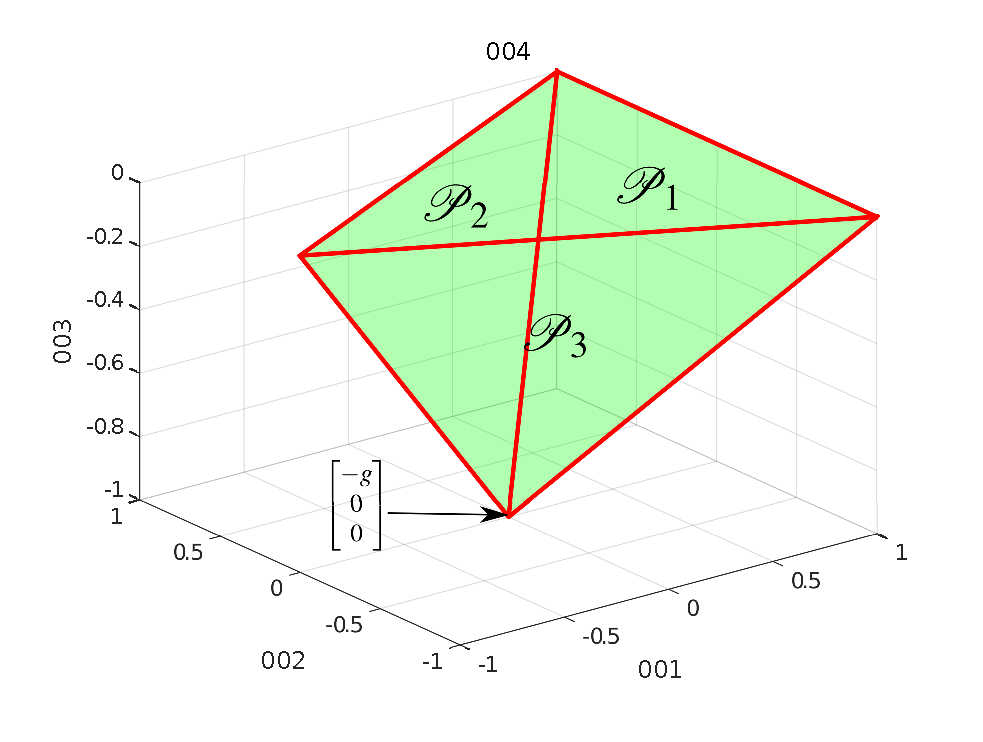
\includegraphics{img/torseur_poly.eps}}
\caption[Tétraèdre des torseurs]{\label{chap1:fig:torseur_poly}Intersections des plans $\mathcal{P}_i$ formant un tétraèdre dans l'espace des composantes du torseur $\mathbfcal{T}$.}
\end{figure}